\section{Methodology}

The workflow is organized as five reproducible screening steps. Step 1 establishes a simplified finite-gain, finite-bandwidth behavioural TIA baseline with explicit total input-node capacitance. Step 2 sweeps feedback capacitance to expose bandwidth and peaking trade-offs. Step 3 maps selected photodiode-capacitance and op-amp bandwidth assumptions into project-defined screening regions. Step 4 quantifies behavioural-vs-vendor-macromodel agreement for selected OP27, OPA818, and ADA4817 export cases. Step 5 adds first-pass behavioural noise context. MATLAB scripts generate the behavioural baseline and parameter sweeps, with outputs stored in the corresponding response and metrics CSV files (Figure~\ref{fig:baseline-response}; Table~\ref{tab:model-assumptions}).

Figure~\ref{fig:methodology-workflow} summarizes the workflow. The process begins by defining design assumptions and parameter ranges, continues through closed-loop behavioural modelling and MATLAB sweep extraction, applies project-defined screening labels, compares selected cases with vendor macromodel exports, and then adds first-pass noise context for design interpretation.

\begin{figure}[H]
  \centering
  \resizebox{0.92\linewidth}{!}{\begin{tikzpicture}[
  block/.style={
    draw,
    rounded corners=1pt,
    align=center,
    text width=10.8cm,
    minimum height=0.88cm,
    inner sep=4pt,
    font=\small
  },
  outputblock/.style={
    draw,
    rounded corners=1pt,
    align=center,
    text width=9.4cm,
    minimum height=0.64cm,
    inner sep=4pt,
    font=\small
  },
  arrow/.style={-{Latex[length=2.2mm]}, line width=0.45pt},
  node distance=0.34cm
]

\node[block] (assumptions) {
  \textbf{1. Define design assumptions}\\[-1pt]
  {\scriptsize $R_f$, $C_f$, $C_{pd}$, $A_0$, $f_t$, $C_{in}$, $C_{\mathrm{stray}}$, supply}
};

\node[block, below=of assumptions] (model) {
  \textbf{2. Behavioural closed-loop TIA model}\\[-1pt]
  {\scriptsize Transfer function and closed-loop response}
};

\node[block, below=of model] (sweeps) {
  \textbf{3. MATLAB sweeps and metric extraction}\\[-1pt]
  {\scriptsize Bandwidth, peaking, gain/phase trends}
};

\node[block, below=of sweeps] (screening) {
  \textbf{4. Project-defined design-region screening}\\[-1pt]
  {\scriptsize Safe / Marginal / Risky classification}
};

\node[block, below=of screening] (vendor) {
  \textbf{5. Vendor macromodel comparison}\\[-1pt]
  {\scriptsize OP27, OPA818, ADA4817}
};

\node[block, below=of vendor] (noise) {
  \textbf{6. First-pass noise screening and design interpretation}\\[-1pt]
  {\scriptsize Noise contribution and trade-off context}
};

\node[outputblock, below=0.42cm of noise] (output) {
  \textbf{Early-stage TIA design-screening workflow}
};

\draw[arrow] (assumptions) -- (model);
\draw[arrow] (model) -- (sweeps);
\draw[arrow] (sweeps) -- (screening);
\draw[arrow] (screening) -- (vendor);
\draw[arrow] (vendor) -- (noise);
\draw[arrow] (noise) -- (output);

\end{tikzpicture}
}
  \caption{Overview of the proposed MATLAB- and vendor-macromodel-assisted workflow for early-stage photodiode TIA design screening.}
  \label{fig:methodology-workflow}
\end{figure}
\FloatBarrier

\ModelAssumptionsTable

\begin{figure}[H]
  \centering
  \begin{subfigure}[t]{0.48\linewidth}
    \centering
    
\includegraphics[width=\linewidth]{figures/tia_baseline_magnitude.png}
    \caption{Magnitude response.}
  \end{subfigure}
  \hfill
  \begin{subfigure}[t]{0.48\linewidth}
    \centering
    
\includegraphics[width=\linewidth]{figures/tia_baseline_phase.png}
    \caption{Phase response.}
  \end{subfigure}
  \caption{Baseline MATLAB behavioural transimpedance response for the selected photodiode TIA case. Panel (a) shows the magnitude response and panel (b) shows the inversion-removed phase response under ideal and finite-gain op-amp assumptions. The curves are behavioural model outputs and are not vendor macromodel or hardware measurement data.}
  \label{fig:baseline-response}
\end{figure}
\FloatBarrier

Step 2 uses the feedback-capacitance sweep to expose the bandwidth and peaking trade-off. Within the selected behavioural sweep, larger $C_f$ reduces extracted bandwidth and generally lowers peaking. This result is interpreted within the explored parameter range, not as a universal compensation law (Figures~\ref{fig:cf-bandwidth} and~\ref{fig:cf-peaking}).

\begin{figure}[H]
  \centering
  
\includegraphics[width=0.75\linewidth]{figures/tia_bandwidth_vs_Cf.png}
  \caption{Extracted $-3$ dB bandwidth versus feedback capacitance for the selected MATLAB behavioural TIA sweep. The figure shows the bandwidth cost associated with increasing $C_f$ under the explored assumptions; it is not a universal compensation rule.}
  \label{fig:cf-bandwidth}
\end{figure}

\begin{figure}[H]
  \centering
  
\includegraphics[width=0.75\linewidth]{figures/tia_peaking_vs_Cf.png}
  \caption{Extracted gain peaking versus feedback capacitance for the selected MATLAB behavioural TIA sweep. Peaking is used here as a project screening metric and stability proxy, not as a complete proof of phase margin or hardware stability.}
  \label{fig:cf-peaking}
\end{figure}
\FloatBarrier

Step 3 maps selected $R_f$, $C_{pd}$, $C_f$, and $f_t$ values into project-defined Safe/Marginal/Risky categories. The criteria and labels are summarized explicitly as project-defined screening definitions (Table~\ref{tab:screening-criteria}). The region map and representative response examples provide the main visual evidence for this stage (Figures~\ref{fig:design-region-map} and~\ref{fig:representative-responses}).

\ScreeningCriteriaTable

\begin{figure}[H]
  \centering
  
\includegraphics[width=0.78\linewidth]{figures/tia_design_region_map_Cpd_ft.png}
  \caption{Project-defined selected-best behavioural design-region map over photodiode capacitance and op-amp transition frequency. Each tile selects the best available feedback capacitance from the behavioural sweep according to the repository's Safe/Marginal/Risky screening labels. The map demonstrates the screening workflow under selected assumptions; its mostly Safe/green appearance should not be interpreted as universal safety or a hardware stability guarantee.}
  \label{fig:design-region-map}
\end{figure}

Figure~\ref{fig:design-region-map} is interpreted as a project-defined selected-best map rather than a universal stability map. A future figure-polish round may pair it with the safe-window fraction map if stronger design-space contrast is needed.

\begin{figure}[H]
  \centering
  
\includegraphics[width=0.78\linewidth]{figures/tia_representative_region_responses.png}
  \caption{Representative MATLAB behavioural transimpedance responses for selected project-defined Safe, Marginal, and Risky cases. The figure connects the screening labels to example frequency-response shapes within the explored assumptions; it does not certify hardware stability.}
  \label{fig:representative-responses}
\end{figure}
\FloatBarrier

\subsection{Behavioural TIA Model}

The behavioural model represents the photodiode TIA as a feedback transimpedance stage with feedback resistance $R_f$, feedback capacitance $C_f$, photodiode capacitance $C_{pd}$, optional op-amp input capacitance $C_{in}$, optional stray input-node capacitance $C_{\mathrm{stray}}$, low-frequency op-amp gain $A_0$, and op-amp transition frequency $f_t$. Table~\ref{tab:model-assumptions} lists the baseline assumptions and swept variables used to produce the manuscript figures.

The feedback impedance is represented as
\begin{equation}
Z_f(s)=\frac{R_f}{1+sR_fC_f},
\end{equation}
and the op-amp is represented by a single-pole finite-gain approximation,
\begin{equation}
A(s)=\frac{A_0}{1+s/\omega_p},
\end{equation}
where $\omega_p=2\pi f_p$ and $f_p=f_t/A_0$. The model defines total input-node capacitance as
\begin{equation}
C_{\mathrm{total}} = C_{pd}+C_{in}+C_{\mathrm{stray}}.
\end{equation}
With an input current source at the summing node and the non-inverting input at AC ground, the closed-loop transimpedance expression used by the behavioural model is
\begin{equation}
\frac{V_{\mathrm{out}}(s)}{I_{\mathrm{in}}(s)} =
\frac{-A(s)Z_f(s)}{1+A(s)+sC_{\mathrm{total}}Z_f(s)}.
\end{equation}
The implementation uses an equivalent admittance form and extracts low-frequency gain, bandwidth, peaking, and phase-related metrics from the resulting response.

This model makes parameter dependence explicit enough for rapid sweep generation. Increasing $C_{\mathrm{total}}$ increases input-node capacitive loading and can reduce bandwidth or increase peaking when the available loop-gain bandwidth is limited. Increasing $C_f$ generally reduces peaking in the explored sweeps but lowers the ideal feedback pole and therefore reduces bandwidth. Increasing $R_f$ raises nominal transimpedance while reducing the ideal feedback pole for a fixed $C_f$. Increasing $f_t$ improves the available loop-gain bandwidth in this single-pole approximation, while $A_0$ affects both low-frequency loop gain and the dominant-pole placement through $f_p=f_t/A_0$.

The model remains a first-order pre-design approximation. It does not reproduce detailed vendor macromodel dynamics, transistor-level behaviour, layout-aware extraction, or measurement. Full-text TIA literature motivates the variables and trade-offs, but the project does not reproduce the circuit methods of Analui 2004, Lu 2007, Noh 2020, or regulated-cascode CMOS TIA papers \citep{ANALUI_2004_BW_ENHANCEMENT,LU_2007_BROADBAND_TIA,NOH_2020_CF_TIA_DC_LOOP,PARK_YOO_2004_RGC_TIA}.

Table~\ref{tab:model-assumptions} is kept as one combined manuscript table in this draft. It combines baseline assumptions, focused feedback-capacitance sweep ranges, full behavioural sweep counts, and design-region evidence layers. Workflow claims are interpreted with respect to their corresponding evidence layers.

\subsection{Design-Region Mapping}

The design-region workflow translates behavioural sweep metrics into project-defined categories. Safe, Marginal, and Risky are internal screening labels, not universal stability classifications and not hardware certification labels. They organize the current sweep results and help select cases for review. Peaking is used as a practical screening metric in this workflow, but it is not by itself a complete phase-margin or stability proof. The map is therefore useful for prioritizing further analysis, not for certifying hardware behaviour.

\subsection{Behavioural-Vs-Vendor Agreement}

Step 4 adds model-specific simulation context by quantifying agreement between the MATLAB behavioural response and OP27, OPA818, and ADA4817 vendor macromodel export summaries under the repository's stated test assumptions. The agreement table reports MATLAB and vendor-export bandwidth, peaking, error values, and project-defined label agreement (Table~\ref{tab:agreement-summary}). A second pass computes each MATLAB case twice, once with $C_{in}=0$ and once with documented vendor-specific $C_{in}$ where available. These comparisons are simulation-only model checks and do not provide experimental validation or complete SPICE coverage.

OPA818 and ADA4817 are treated as the main high-speed agreement cases. The key pattern is that agreement is strongest at moderate and larger $C_f$ values, while the smallest-$C_f$ rows behave as boundary cases. For OPA818, all four selected vendor rows agree with the MATLAB behavioural model in the project-defined label comparison, but bandwidth error is largest at the smallest feedback capacitance and decreases for moderate and larger $C_f$ values. For ADA4817, three of four rows agree in the project-defined label comparison; the smallest-$C_f$ row remains a cautionary case where the vendor macromodel reports more peaking than the simplified behavioural model.

OP27 is retained as a low-GBW negative-control and illustrative limitation case. The smallest-$C_f$ OP27 row disagrees in the project-defined label comparison and shows a large peaking mismatch. This behaviour is useful because it exposes how a simplified single-pole behavioural model and uncertain input-capacitance assumptions can diverge from a vendor macromodel in a low-GBW case. OP27 is therefore not presented as primary high-speed TIA evidence.

The Round 28 Cin ablation is interpreted as a model-scope check rather than an accuracy claim. In the current vendor rows, $C_{pd}=10$ pF dominates the documented $C_{in}$ values, so the ablation shows mixed and modest bandwidth-error changes rather than a uniform improvement. The documented-Cin pass improves the ADA4817 aggregate bandwidth-error metric but worsens the OPA818 aggregate metric under the current single-pole assumptions; label agreement is unchanged.

The agreement evidence should be interpreted as screening-level model agreement. It supports the workflow claim that behavioural screening and vendor macromodel summaries can be compared quantitatively, while also showing that small-$C_f$ cases remain model-sensitive.

\AgreementSummaryTable

\begin{figure}[H]
  \centering
  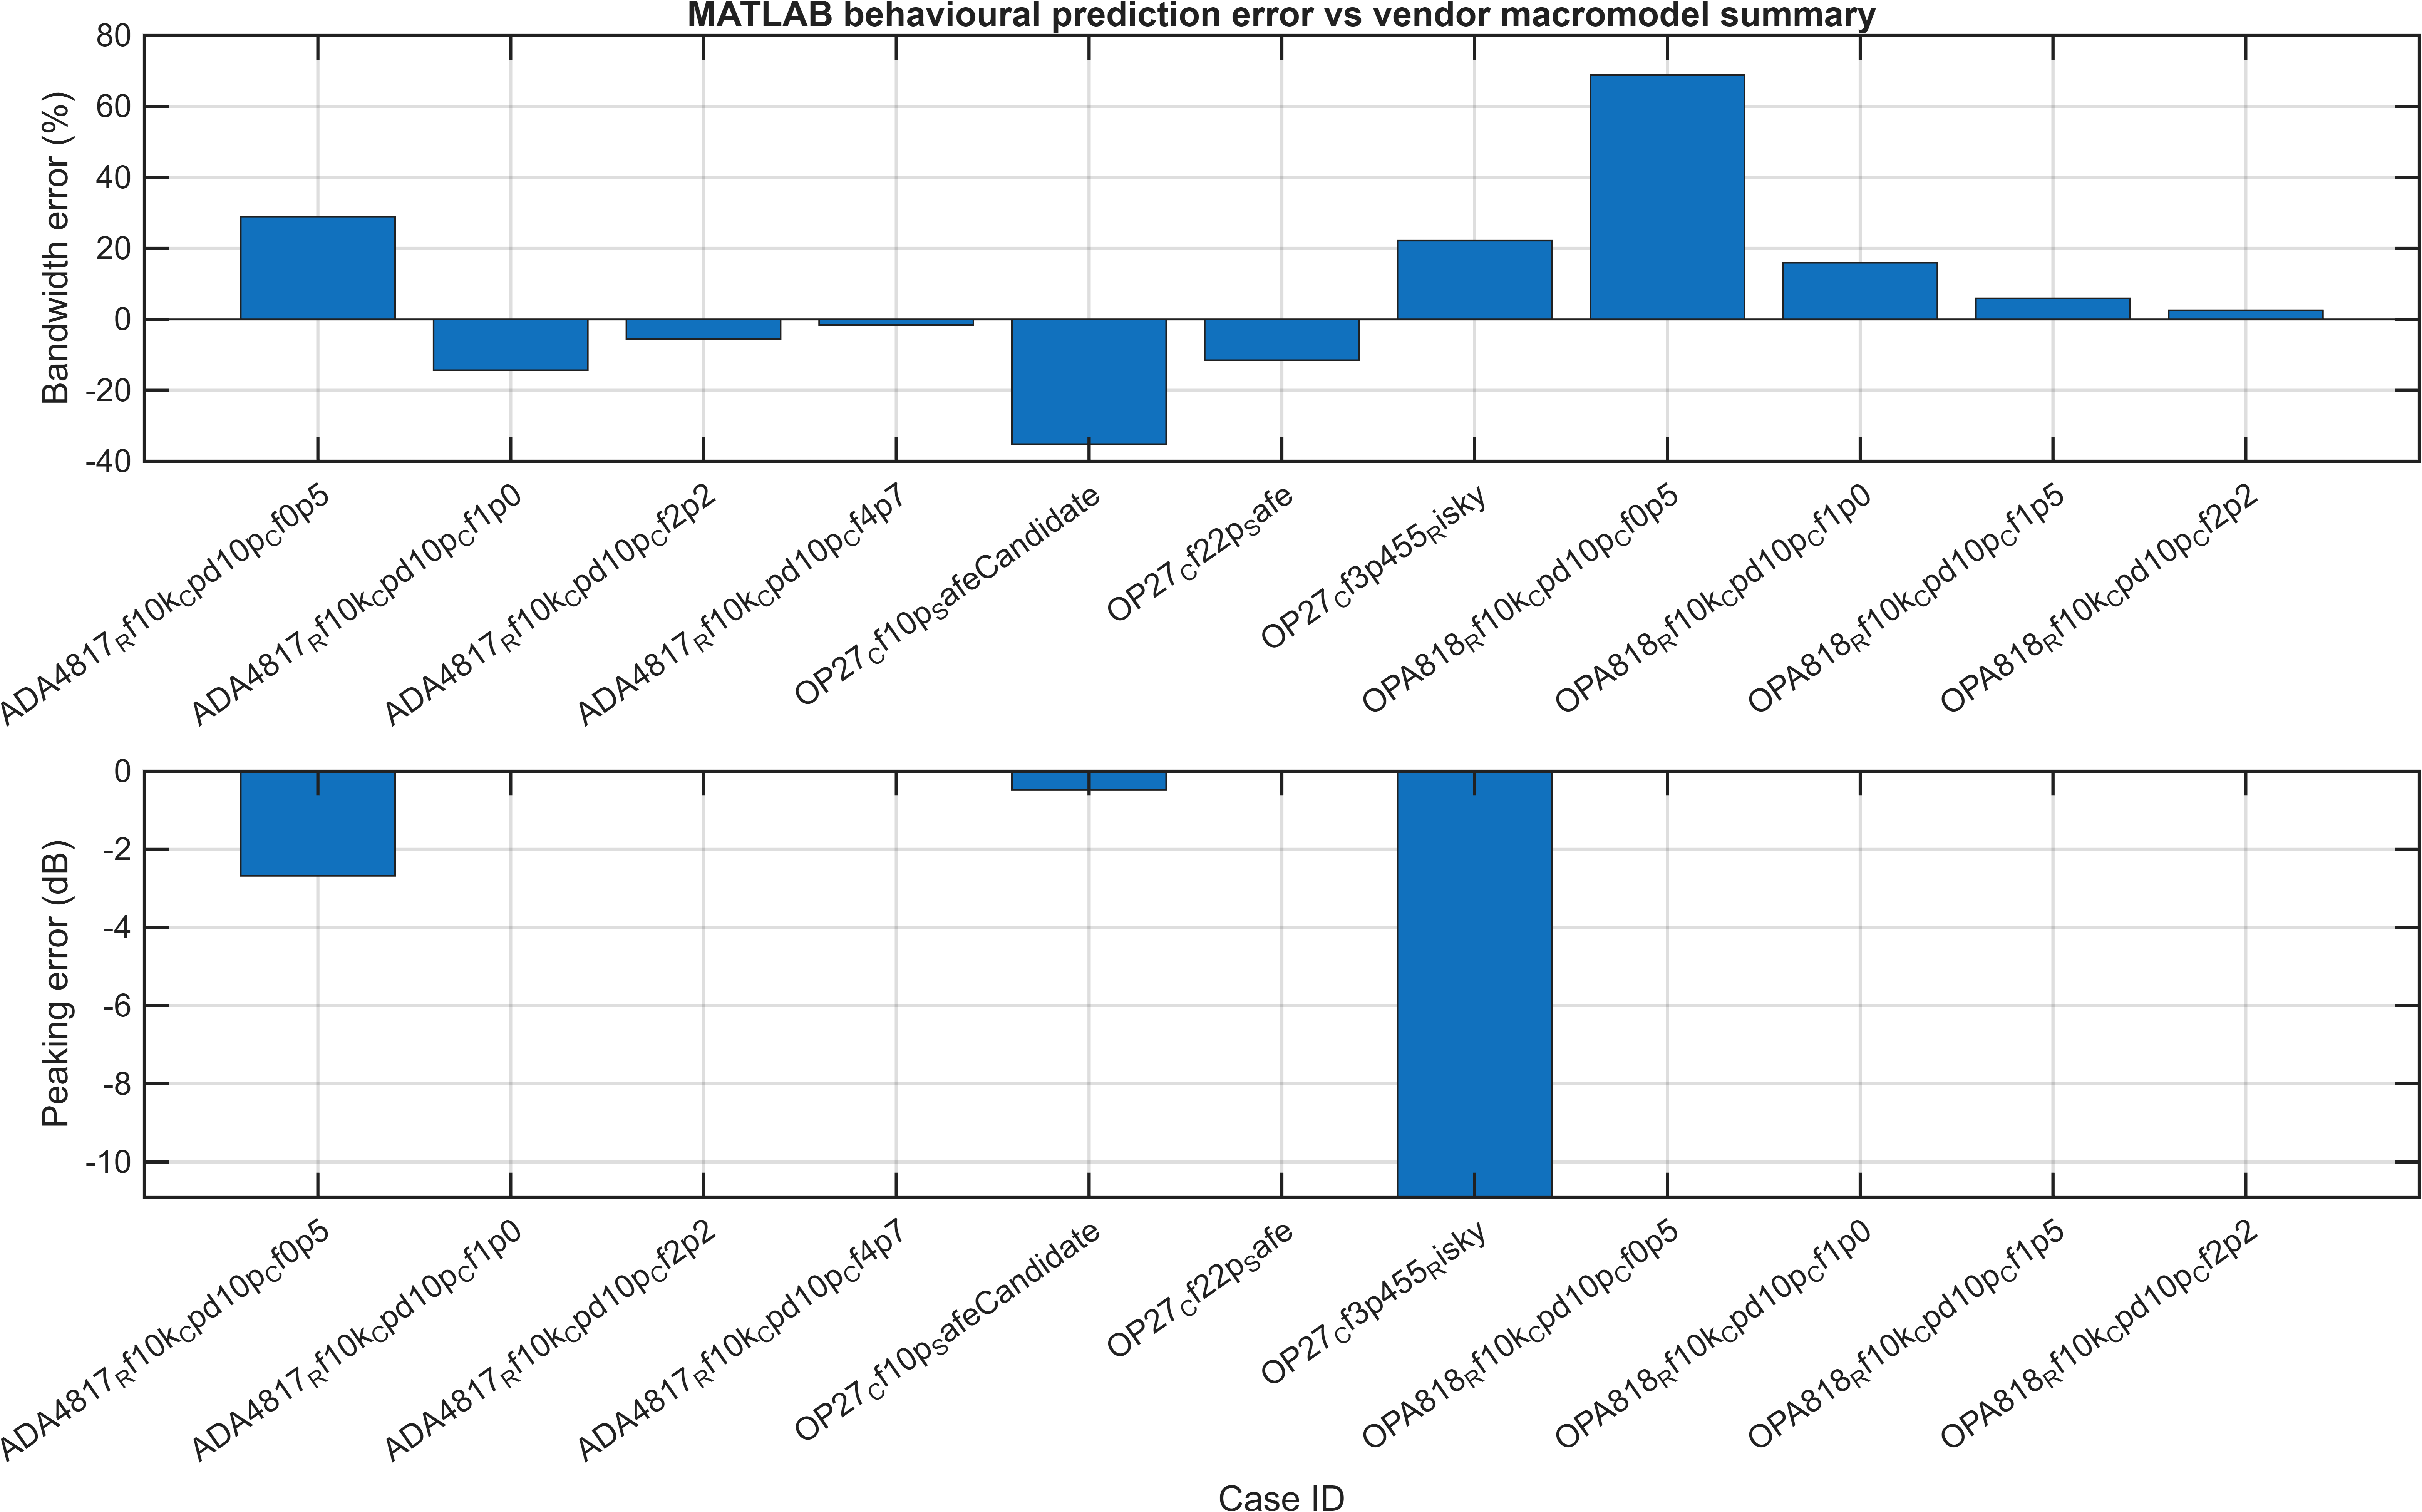
\includegraphics[width=0.84\linewidth]{figures/behavioural_vs_vendor_agreement_error_summary.png}
  \caption{Behavioural-vs-vendor-macromodel agreement error summary for OP27, OPA818, and ADA4817 feedback-capacitance cases. Bandwidth error is computed as $100(\mathrm{MATLAB}-\mathrm{vendor})/\mathrm{vendor}$, and peaking error is MATLAB peaking minus vendor peaking.}
  \label{fig:model-agreement-error-summary}
\end{figure}
\FloatBarrier

\subsection{First-Pass Noise Analysis}

Step 5 extends the bandwidth and peaking discussion by estimating relative noise contributions under configured assumptions. The first-pass behavioural noise model includes configured feedback resistor, op-amp voltage-noise, op-amp current-noise, and photodiode shot-noise terms. The baseline contribution figure summarizes the configured output-noise terms for the baseline behavioural case (Figure~\ref{fig:noise-baseline}).

These outputs are first-pass behavioural estimates. They are not measured noise, detector-complete noise validation, or SPICE noise analysis. Their purpose is to show how the same workflow can carry noise assumptions into the screening discussion when compensation choices change. The noise-bandwidth trade-off figure connects this estimate back to the compensation sweep (Figure~\ref{fig:noise-tradeoff}).

The literature supports the relevance of discussing noise and bandwidth together. Noh 2020 supports capacitive-feedback and noise/stability context \citep{NOH_2020_CF_TIA_DC_LOOP}. Lu 2007 and Abdollahi 2025 support broad-band and noise-aware TIA framing \citep{LU_2007_BROADBAND_TIA,ABDOLLAHI_2025_MDFRGC_TIA}.
% TODO citation pending manual check: LI_2021_LOW_NOISE_OPTICAL_RX_TIA is excluded from references_draft.bib.
